\documentclass{article}
\usepackage{color}
\usepackage{graphicx}
\usepackage[caption=false]{subfig}
\usepackage{amsmath}
\usepackage{amsthm}
\usepackage{amsfonts}
\usepackage{mathtools}
\usepackage{cleveref}
\usepackage[utf8]{inputenc}
\usepackage{algpseudocode}
\usepackage{algorithm}

\graphicspath{{figures/}}

% Environments
\newtheorem{theorem}{Theorem}
\newtheorem{definition}{Definition}
\newtheorem{problem}{Problem}
\newtheorem{remark}{Remark}

% Aliases

\newcommand*{\xd}{\dot{x}}
\newcommand*{\R}{\mathbb{R}}
\newcommand*{\N}{\mathbb{N}}

%% Temporal logic symbols
% \newcommand{\not}{\neg}
% \newcommand{\and}{\wedge}
% \newcommand{\or}{\vee}
\newcommand{\Next}{\mathbf{X}}
\newcommand{\Always}{\mathbf{G}}
\newcommand{\Event}{\mathbf{F}}
\newcommand{\luntil}{\mathbf{U}}
\newcommand{\Implies}{\Rightarrow}
\newcommand{\Not}{\lnot}
\newcommand{\True}{\top}

% \newcommand*{\iff}{\Leftrightarrow}

\newcommand*{\psat}[1]{[[#1]]}

\newcommand*{\fran}[1]{\textcolor{blue}{#1}}

\title{Placeholder}

\author{Francisco Penedo}

\begin{document}

\section{Introduction}
\label{sec:introduction}

\section{Preliminaries}
\label{sec:preliminaries}

\subsection{Heat Equation and Finite Element Analysis}
\label{sub:heat_equation_and_finite_element_analysis}

Let $\Omega = (0, L) \subset \R$ be an open interval representing the interior
of a one-dimensional rod of length $L$; $\rho, c, \kappa > 0$ 
constants denoting density, capacity and conductivity of the rod's material respectively;
$g_0, g_L \in \R$ the boundary conditions at each end of the rod; and $u_0 :
\Omega \rightarrow \R$ an initial value for the temperature on the rod. 
The evolution of the temperature at
each point in the rod can be described by a function $u : \bar \Omega \times [0,
T] \rightarrow \R$, where $T > 0$ denotes the final time and can be infinity, 
such that the following equations are satisfied:

\begin{equation}\label{eq:pde}
    \begin{aligned}
        \rho c \frac{\partial u}{\partial t} - \kappa \frac{\partial^2
        u}{\partial^2 x} &= 0, \text{on } \Omega \times (0, T) \\
        u(0, t) &= g_0, \forall t \in (0, T) \\
        u(L, t) &= g_L, \forall t \in (0, T) \\
        u(x, 0) &= u_0(x), \forall x \in \Omega
    \end{aligned}
\end{equation}

In the following we will call $\Sigma$ a system governed by \eqref{eq:pde},
described by the parameters $L, \rho, c$ and $\kappa$, and with boundary
conditions $g_0, g_L$.


Let $\{x_i\}_{i = 0}^{n +
1}$, where $x_0 = 0, x_{n+1} = L, x_i \in \Omega, i = 1,...,n$, be a partition of
$\bar\Omega$. Let $d_i(t), i = 0,...,n+1$ represent the
temperature of the rod at the point $x_i$, with $d_0(t) = g_0, d_{n+1} = g_L$ and let $d = (d_1, ..., d_n)' \in
\R^n$. We define the following linear node shape function matrices for $i =
0,...,n+1$:

\begin{equation}
    N_i(x) = \begin{cases}
        \frac{x - x_{i - 1}}{x_i - x_{i - 1}} & i > 0, x \in [x_{i-1}, x_i] \\
        \frac{x_{i+1} - x}{x_{i+1} - x_{i}} & i < n+1, x \in [x_{i}, x_{i+1}] 
    \end{cases} 
\end{equation}

and the following linear interpolation of $d$:

\begin{equation}
    u^d(x, t) = \sum_{i=0}^{n+1} N_i(x) d_i(t)
\end{equation}

It can be shown\footnote{\fran{At some point I'll fill in the details of the
construction of $A$ and $b$}} that $u^d(x, t)$ is a good approximation of 
$u(x, t)$, where $u(x,t)$ is the trajectory of $\Sigma$ for an
initial value $u_0$, and $d$ evolves
according to the following linear system, $\Sigma_{FEM}$:

\begin{equation}\label{eq:fem}
    \begin{aligned}
        \dot{d} &= A d + b
    \end{aligned}
\end{equation}

with initial value $d_i(0) = u_0(x_i), i = 1,...,n$. In the above, $A$ is a
banded matrix of bandwidth 3. We call $\Sigma_{FEM}$ the FEM system
corresponding to system $\Sigma$.


\section{Signal Temporal Logic for PDEs}
\label{sec:signal_temporal_logic}

In this section we define a bounded time linear temporal logic suitable to
define specifications for solutions of partial differential equations. We start
by defining standard Signal Temporal Logic (STL) and then defining a new set of
predicates over both spatial- and time-varying signals.

An STL formula $\phi$ is defined recursively in the following way:

\begin{equation}
    \phi ::= \mu | \lnot \mu | \phi_1 \land \phi_2 | \phi_1 \luntil_{[a,b]} \phi_2
\end{equation}

where $\mu$ is a predicate over signals of the form $\mu \equiv \mu(s) > 0$,
$\phi_1$ and $\phi_2$ are STL formulas,
$\lnot$ and $\land$ are the Boolean operators negation and conjunction, and
$\luntil_{[a, b]}$ is the bounded temporal operator \emph{until}. The satisfaction
of an STL formula at time $t$ for a signal $s :
\mathbb{T} \to \R$, where $\mathbb{T}$ is a discrete or continuous time domain
and $t \in \mathbb{T}$, is defined recursively as follows:

\begin{equation}
    \begin{aligned}
        s[t] &\models \mu &\iff &\mu(s(t)) > 0 \\
        s[t] &\models \lnot \mu &\iff &\lnot (s[t] \models \mu) \\
        s[t] &\models \phi_1 \land \phi_2 &\iff &s[t] \models \phi_1 \land s[t]
        \models \phi_2 \\
        s[t] &\models \phi_1 \luntil_{[a,b]} \phi_2 &\iff 
            &\exists t' \in [t+a, t+b] \text{ s.t. } s[t'] \models \phi_2 \\
        & & &\land \forall t'' \in [t, t'] s[t''] \models \phi_1]
    \end{aligned}
\end{equation}

In the above equation, the time intervals are to be understood inside
$\mathbb{T}$. A signal $s$ satisfies an STL formula, $s \models \phi$, if and
only if $s[0] \models \phi$. We define other Boolean operators (disjunction,
implication and equivalence) and constants (true and false) in the usual way, 
and the temporal operators
\emph{eventually} and \emph{globally} as $\Event_{[a, b]} \phi \equiv \top
\luntil_{[a,b]} \phi$ and $\Always_{[a, b]} \phi \equiv \lnot \Event_{[a,b]}
\lnot \phi$ respectively.

We also define quantitative semantics for STL formula over a signal $s$
using the real valued function $r(\phi, s, t)$, which satisfies the property $s[t]
\models \phi \iff r(\phi,s, t) > 0$ and is computed as follows:

\begin{equation}
    \begin{aligned}
        &r(\mu, s, t) &= &\mu(s(t)) \\
        &r(\lnot \mu, s, t) &= &-r(\mu, s,t) \\
        &r(\phi_1 \land \phi_2, s, t) &= &\min\{r(\phi_1,s, t),
    r(\phi_2,s, t)\} \\
    &r(\phi_1 \luntil_{[a,b]} \phi_2,s, t) &= 
    &\max_{t' \in [t+a, t+b]} \left \{ \min\{ r(\phi_2,s, t), 
\min_{t'' \in [t, t']}\{r(\phi_1,s, t)\}\} \right \}
    \end{aligned}
\end{equation}

We call $r(\phi,s, t)$ the robustness degree of $s$ with respect to $\phi$ at
time $t$.

In order to define STL for PDEs, we introduce the following set of predicates:
let $\Lambda = \{\lambda_i | i = 1,...,m\}$ be a set of predicates, where
$\lambda_i$ is a predicate represented as a tuple $(Q_i, X_i, \mu_i)$, and informally represented using the syntax $``Q_i x \in X_i : u(x) - \mu_i(x) >
0"$, where:

\begin{itemize}
    \item $Q_i \in \{\forall, \exists\}$ is the spatial quantifier,
    \item $X_i \subseteq \bar\Omega$ is the spatial domain of the predicate and
        we require it to be a closed set, and 
    \item $\mu_i : X_i \to \R$ is a continuous and differentiable function 
        representing the reference profile.
\end{itemize}

We will sometimes use $Q_\lambda, X_\lambda, \mu_\lambda$ to refer to the
elements of the tuple representing $\lambda$. We consider STL formulas 
with the previously defined syntax and semantics 
over the set of predicates $\Lambda$, where the satisfaction of a
predicate with respect to a continuous-time signal $u : \bar\Omega \times [0, T]
\to \R$ at time $t \in \R$ is defined as $u[t] \models \lambda_i \iff 
u(x, t) - \mu_i(x) > 0$ for all $x \in X_i$ if $Q_i = \forall$ or for some $x \in
X_i$ otherwise. We define the quantitative semantics as before with
$r(\lambda_i,u, t) = \min_{x \in X_i} u(x, t)$ if $Q_i = \forall$ and
$r(\lambda_i,u, t) = \max_{x \in X_i} u(x, t)$ otherwise.

\section{Problem Formulation}
\label{sec:problem_formulation}

We can formulate now the STL verification problem for trajectories of a heat
equation:

\begin{problem}
\label{pr:stl}
    Given a system $\Sigma$, an STL formula $\psi$ and initial state $u_0$,
    check wether the trajectory of $\Sigma$ for the initial state $u_0$
    satisfies $\psi$ at time 0.
\end{problem}

A more general problem can be formulated if we consider the initial state to be
in a set:

\begin{problem}
\label{pr:stl_set}
    Given a system $\Sigma$, an STL formula $\psi$ and a set of initial states
    $U_0$, check wether the trajectory of $\Sigma$ satisfies $\psi$ at time 0
    for any initial state $u_0 \in U_0$.
\end{problem}

In order to solve both problems, we first reformulate the specification $\psi$
in such a way that it allows us to solve the verification problems
conservatively on a discrete time linear system instead.

\section{Formally Correct Discretization of STL for PDEs}
\label{sec:formally_correct_discretization_of_pdestl}

We first reformulate the specification $\psi$ so that we can verify instead the
approximation given by $\Sigma_{FEM}$. Recall that we denote as $u(x,t)$ the
trajectory of $\Sigma$ and $u^d(x, t)$ the piecewise linear approximation
obtained by interpolating the trajectory of $\Sigma_{FEM}$. In the following, we
assume the partition $\{x_i\}_{i=1}^m$ is proposition preserving with respect 
to the set of
regions $\{X_i\}_{i = 1}^{m}$\footnote{This is well defined since the $X_i$ are
closed and there are a finite number of them}. Suppose we are given
an a priori bound, $\epsilon(x, t)$, on the pointwise difference between them, i.e., 
$|u(x, t) - u^d(x, t)| \leq \epsilon(x, t)$.

\begin{definition}
\label{def:m_perturbation}
    Let $\lambda \in \Lambda$ be the predicate represented by the tuple $(Q, X,
    \mu)$ and let $M : \bar\Omega \to \R$ be a continuous function. The perturbation of
    $\lambda$ by $M$, $\lambda^M$, is the predicate given by the tuple $(Q, X,
    \mu^M)$, where $\mu^M(x, u) = \mu(x, u) + M(x)$.
\end{definition}

\begin{definition}
\label{def:delta_perturbation}
    Let $\psi$ be an STL formula over $\Lambda$ in negation normal form 
    and let $\delta : \bar\Omega \to \R$ be a continuous function. The
    conservative perturbation of $\psi$ by $\delta$, $\psi^\delta$, is an STL
    formula in negation normal form obtained by substituting every predicate
    $\lambda$ that appears in $\psi$ and is represented by $(Q, X, \mu)$ in the
    following way:

    \begin{itemize}
        \item If $\lambda$ is not preceded by a negation operator, then it is
            substituted by $\lambda^{-\delta}$.
        \item Otherwise, it is substituted by $\lambda^{\delta}$
    \end{itemize}

    We will also use $\Lambda^{\delta}$ to refer to the set of all $\delta$ and
    $-\delta$
    perturbations of predicates in $\Lambda$.
\end{definition}

\begin{theorem}
\label{th:epsilon_approximation}
    If $u^d \models \psi^{\delta}$, with $\delta(x) = \max_t \epsilon(x, t)$, then $u \models \psi$.
\end{theorem}
\begin{proof}
    We only need to consider a predicate $\lambda$ and its negation. We have
    \begin{equation}
        \label{eq:th_epsilon}
         |u(x, t) - \mu_\lambda(x) - u^d(x, t) + \mu_\lambda(x)| = 
         |u(x, t) - u^d(x, t)| \leq \delta(x)
    \end{equation}
    Thus, $u(x, t) - \mu_\lambda(x) \geq u^d(x, t) -
    \mu_\lambda(x) - \delta(x)$, which proves the result for $\psi = \lambda$. For $\psi
    = \lnot \lambda$, note that satisfaction is equivalent to $u(x, t) -
    \mu_\lambda(x) < 0$ for $x$ quantified opposite to $Q_\lambda$. Then, from
    \eqref{eq:th_epsilon} we have $u(x, t) - \mu_\lambda(x) \leq u^d(x, t) +
    \mu_\lambda(x) - \delta(x)$, completing the proof.
\end{proof}

Theorem~\ref{th:epsilon_approximation} gives us a way to conservatively solve
Problem~\ref{pr:stl} using the approximation obtained from $\Sigma_{FEM}$.
However, we still need to deal with continuous functions in continuous time. Our
next step will be to reformulate the problem into a verification problem over
the trajectory of $\Sigma_{FEM}$, i.e., $d(t)$.

Let $\Lambda^{\delta}_{FEM} = \{\alpha_{\lambda, j} | \lambda \in
\Lambda^{\delta}, e \in E_{\lambda}\} \cup \{\beta_{\lambda, j} | \lambda \in
\Lambda^{\delta}, j \in J_{\lambda}\}$, where $E_{\lambda} = \{e | [x_e, x_{e+1}] \subseteq
X_{\lambda}\}, J_{\lambda} = \{j | x_j \in X_\lambda, [x_{j-1}, x_j] \not\subseteq
X_\lambda, [x_{j}, x_{j+1}] \not\subseteq X_\lambda \}$,
and satisfaction of $\alpha_{\lambda, e}$ and $\beta_{\lambda, j}$ by 
for a continuous-time signal $d : [0, T] \to \R^n$
is defined in the following way  

\begin{equation}
    d[t] \models \alpha_{\lambda, e} \iff y_e(t) - 
    \mu_\lambda(\frac{x_e + x_{e + 1}}{2}) > 0 
\end{equation}
\begin{equation}
     d[t] \models \beta_{\lambda, j} \iff d_j(t) - \mu_\lambda(x_j) > 0
\end{equation}

where $y_e = \frac{d_e(t) + d_{e+1}(t)}{2}$. The robustness degree for these
predicates is defined as in Sec.~\ref{sec:signal_temporal_logic}.
Note that this set of predicates includes the perturbations defined in
Def.~\ref{def:delta_perturbation}. We define perturbations of predicates in
$\Lambda^{\delta}_{FEM}$ by a real number $K$ in a manner analogous to
Def.~\ref{def:m_perturbation}, and we denote it as $\alpha^K$.

\begin{definition} 
\label{def:eta_approximation}
    The STL formula over $\Lambda^{\delta}_{FEM}$, $\psi^{\delta, \eta}_{FEM}$, corresponding to an STL
    formula in negation normal form, $\psi^\delta$, over $\Lambda^\delta$, with
    $\eta : \bar\Omega \to \R$, is a formula obtained by substituting every
    predicate $\lambda$ in $\psi^\delta$ by the formula $\bigoplus_{e \in
    E_\lambda} \gamma_{\lambda,e} \oplus \bigoplus_{j \in J_\lambda} \beta_{\lambda, j}$, 
    where $\oplus = \wedge$ if $Q_i = \forall$ and $\oplus = \vee$
    otherwise, and $\gamma_{\lambda,e}$ is defined as the following STL formula:

    \begin{itemize}
        \item If $\lambda$ is not preceded by a negation operator, then
            $\gamma_{\lambda, e} = \alpha_{\lambda, e}^{-K_e}$.
        \item Otherwise, $\gamma_{\lambda, e} = \alpha_{\lambda, e}^{K_e}$.
    \end{itemize}

    In both cases, 

    \begin{equation}
    \begin{aligned}
        K_e = \frac{x_{e+1} - x_e}{2} & \left (\max_{c \in [x_e, x_{e+1}]}
        |\mu'(c)| + \max_{c \in [x_e, x_{e+1}]} \eta(c) \right )
    \end{aligned}
    \end{equation}

    We will abuse the notation and use $\psi^{\delta, 0}_{FEM}$ when referring
    to the formula obtained without perturbing the predicates, i.e., both $\eta$
    and $\mu'$ are considered 0.
\end{definition}
% \frac{\partial u}{\partial x}(c, t)

\begin{theorem}
\label{th:eta_approximation}
    If $d \models \psi^{\delta, \eta}_{FEM}$, with $\eta(x) \geq \max_t |\frac{\partial
    u^d}{\partial x}(x, t)|$, then $u^d \models \psi^\delta$.
\end{theorem}
\begin{proof}
    We only need to consider a predicate $\lambda$ and its negation. We assume
    $Q_\lambda = \forall$, the other case is similar. Let $X_\lambda = [x_a,
    x_b]$. First note that satisfying $\lambda$ is equivalent to satisfying all
    predicates of the set $\{(Q_\lambda, [x_e, x_{e+1}], \mu_\lambda) | e \in
    E_\lambda\}$. For any $e \in E_\lambda$, let $m = \frac{x_e + x_{e+1}}{2}, 
    h = \frac{x_{e+1} - x_{e}}{2}$. 
    For $x \in [x_e, x_{e+1}]$ we have:

    \begin{equation}
    \begin{aligned}
        &|u^d(x, t) - \mu_\lambda(x) - u^d(m, t) + \mu_\lambda(m)| \leq \\
        &h \max_{c \in [x_e, x_{e+1}]} 
        |\mu'(c) + \frac{\partial u^d}{\partial x}(c, t)|
        \leq \\
        &h \left (  
        \max_{c \in [x_e, x_{e+1}]} |\mu'(c)| +
        \max_{c \in [x_e, x_{e+1}]} |\frac{\partial u^d}{\partial x}(c, t)|
        \right ) \leq \\
        &h \left (  
        \max_{c \in [x_e, x_{e+1}]} |\mu'(c)| +
        \max_{c \in [x_e, x_{e+1}]} \eta(c)
        \right )  = K_e
    \end{aligned}
    \end{equation}

    Then, $u^d(x, t) - \mu_\lambda(x) \geq u^d(m, t) - \mu_\lambda(m) - K_e =
    y_e(t) - \mu_\lambda(m) - K_e$, so $d \models \alpha^{-K_e}_{\lambda, e}$
    implies $u^d \models (Q_\lambda, [x_e, x_{e+1}], \mu_\lambda)$ and the
    theorem holds for $\psi^\delta = \lambda$. To prove it for the negated
    predicate, we can follow an argument similar to the one in the proof of
    Th.~\ref{th:epsilon_approximation}.
\end{proof}

Finally, we reformulate the problem into a verification problem over the
trajectory of a time discretization of $\Sigma_{FEM}$. Let $\Delta t \in \R$ be
a positive time interval. The discretization of $\Sigma_{FEM}$ with time
interval $\Delta t$, $\Sigma^{\Delta t}_{FEM}$, is a system that evolves
according to the following difference equation:

\begin{equation}
    \begin{aligned}
        \tilde d^{k+1} &= \tilde A \tilde d^k + \tilde b \\
        \tilde d^0 &= d(0)
    \end{aligned}
\end{equation}

where $\tilde A = e^{A \Delta t}$ and $\tilde b = - e^{A \Delta t} A^{-1} \left
( e^{- A \Delta t} - I \right ) b$. Note that $d(k \Delta t) = \tilde d^k,
\forall k \in \N$. 
% We define satisfaction of an STL formula by a discrete time
% signal in a similar way to continuous time. However, we make a slight abuse of
% notation so that the time bounds for the temporal operators should be understood
% in the continuous sense, i.e, $\tilde d[k] \models \Always_{[a, b]} \psi \iff 
% \forall j \in [\frac{a}{\Delta t}, \frac{b}{\Delta t}] \cap \N, \tilde d^{k + j} \models
% \psi$ and similarly with the eventually operator.

We define a conservative perturbation of $\psi^{\delta, \eta}_{FEM}$ by a real
vector $\nu = (\nu^y, \nu^d)$, $\psi^{\delta, \eta, \nu}_{FEM}$, in a similar
way to Def~\ref{def:eta_approximation}, noting that the predicate $\gamma_{\lambda, e}$ is perturbed
using the constant $L_e^y = \Delta t \nu^y_e$ and the predicate $\beta_{\lambda, j}$ is
perturbed using the constant $L_j^d = \Delta t \nu^d_j$.

\begin{theorem}
    \label{th:nu_approximation}
    If $\tilde d \models \psi^{\delta, \eta, \nu}_{FEM}$, with
    $\nu^y_e = \max_t \frac{|\dot d_e(t)| + |\dot d_{e+1}(t)|}{2}$ and $\nu^d_j = \max_t
    |\dot d_j(t)|$, then $d \models \psi^{\delta, \eta}_{FEM}$.
\end{theorem}
\begin{proof}
    Similar to Th.~\ref{th:eta_approximation}.
\end{proof}

Using Theorem~\ref{th:nu_approximation} we can solve Problem~\ref{pr:stl}
conservatively by solving a verification problem for regular STL and discrete
time linear systems. Moreover, we can obtain a bound on the robustness of the
original specification with respect to the trajectory of $\Sigma$ by making the
following observation:

\begin{theorem}
    \label{th:robustness}
    If $u, u^d, d$ and $\tilde{d}$ are trajectories of $\Sigma$, interpolation
    of $\Sigma_{FEM}$, $\Sigma_{FEM}$ and $\Sigma_{FEM}^{\Delta t}$,
    respectively, and $\psi$ is an STL formula over $\Lambda$, then the 
    following inequality holds:

    \begin{equation}
        r(\psi, u, t) \geq r(\psi^{\delta}, u^d, t) \geq r(\psi^{\delta, \eta},
        d, t) \geq r(\psi^{\delta, \eta, \nu}, \tilde{d}, t)
    \end{equation}
\end{theorem}
\begin{proof}
    It follows from the proofs of
    \cref{th:epsilon_approximation,th:eta_approximation,th:nu_approximation}.
\end{proof}

\section{Verification of Initial Sets}
\label{sec:verification_of_initial_sets}

\section{Examples}
\label{sec:examples}

We consider first the verification of a single initial value using uniform
meshes of different sizes. Consider a rod with parameters given in
Table~\ref{tab:ex_pars}, initial value $u_0(x) = 20.0$
for $x \in (0, L)$, $u_0(0) = g_0, u_0(L) = g_L$, and the following specification:

\begin{equation}
    \psi = \Always_{[1,10]} ``\forall x \in [8,9] : u(x) - (28x - 192) > 0"
\end{equation}

which reads in natural language: ``Always between 1 and 10 time units, all
points in the rod between lengths 8 and 9, the temperature profile is above the
profile $\mu(x) = 28x - 192$." Note that we used the informal syntax for
predicates to improve the readability of the formula. We show in
Fig.~\ref{fig:ex1_evolution} the trajectory for two mesh sizes along with the
profile in the specification.

\begin{figure}[!t]
    \centering 
    \subfloat[$h = 1.0$]{\label{fig:ex1_a}
        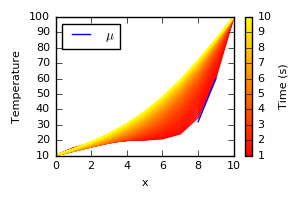
\includegraphics[width=0.49\textwidth]{ex1_plots10.png}}
        \hfill
    \subfloat[$ h = 0.2$]{\label{fig:ex1_b}
        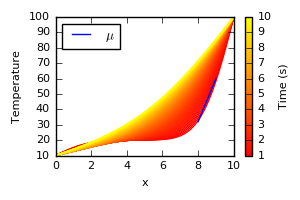
\includegraphics[width=0.49\textwidth]{ex1_plots50.png}}
        \hfill
    \caption{Trajectory $u^d(x, t)$ for two mesh sizes and the reference
        temperature profile $\mu(x) = 28x - 192$. Note how the trajectory
        obtained with a coarser mesh satisfies the specification, while the one
        obtained with a finer mesh does not.}
    \label{fig:ex1_evolution}
\end{figure}


\begin{table}
\centering
\begin{tabular}{|c|c|c|c|c|c|c|}
    \hline
    & $L$ & $\rho$ & $c$ & $\kappa$ & $g_0$ & $g_L$ \\
    \hline
    Rod 1 & 10 & 1 & 1 & 1 & 10 & 100 \\
    \hline
\end{tabular}
\caption{Rod parameters}
\label{tab:ex_pars}
\end{table}

Throughout this
section we will consider the true trajectory of the system for some initial
value, $u^*(x, t)$, the solution of the associated FEM system with a uniform mesh of
size $h = 0.01$.

We computed the bound $\delta(x) = \delta$ as the maximum pointwise
error between simulations of the true trajectory and the trajectory for the
given mesh using random initial values of the form $u_0(x) = \min\{\max\{a x +
b, g_0\}, g_L\}$ with $|a| < 2 |g_L - g_0| / L$ and $b \in (0, |g_L - g_0|)$.
Likewise, we determined the bounds $\eta(x)$ and $\nu$ from those simulated
trajectories. We show in Fig.~\ref{fig:bounds} the resulting bounds for two mesh
sizes.

\begin{figure}[!t]
    \centering 
    \subfloat[$h = 0.5$]{\label{fig:bounds_a}
        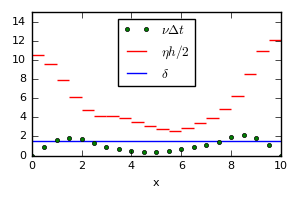
\includegraphics[width=0.49\textwidth]{pert_plot_N20.png}}
        \hfill
    \subfloat[$ h = 0.2$]{\label{fig:bounds_b}
        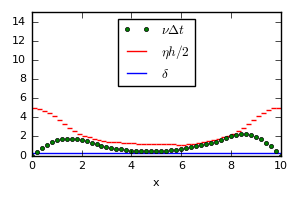
\includegraphics[width=0.49\textwidth]{pert_plot_N50.png}}
        \hfill
    \caption{Bounds used for $\delta$, $\eta$ and $\nu$ multiplied by their
    respective coefficients in the perturbation terms. Note that we show $\nu^d_j$ at
    $x_j$ and use $\nu_e^y = \frac{\nu^d_j + \nu^d_{j+1}}{2}$}
    \label{fig:bounds}
\end{figure}

The robustness results are shown in Table~\ref{tab:res_meshes}. As expected, finer meshes
yield robustness values closer to the true robustness.

\begin{table}
\centering
\begin{tabular}{|c|c|c|c|c|c|c|}
    \hline
    $h$ & $\delta$ & $r(\psi_{FEM}^{0, 0, 0})$ & $r(\psi_{FEM}^{\delta, 0, 0})$ &
    $r(\psi_{FEM}^{\delta, \eta, 0})$ & $r(\psi_{FEM}^{\delta, \eta,
\nu})$ & Time (s)  \\
    \hline
    1 & 5.29 & 1.66 & -3.44 & -32.25 & -34.10 & 0.5 \\
    0.5 & 1.49 & -1.57 & -2.93 & -18.61 & -20.61 & 1.5 \\
    0.33 & 0.68 & -2.29 & -2.92 & -13.34 & -15.47 & 3.6 \\
    0.25 & 0.37 & -2.68 & -3.03 & -10.55 & -12.72 & 5.9 \\
    0.2 & 0.24 & -2.74 & -2.94 & -9.10 & -11.27 & 9.9 \\
    \hline
\end{tabular}
\caption{Verification of a single initial value. Robustness of the true
trajectory is -2.7}
\label{tab:res_meshes}
\end{table}

We checked the validity of our approach as well as the degree of
conservativeness that the perturbations add by verifying random initial values
of the previous form. We used for this example a uniform mesh of size $h = 0.2$
and the following specification: 

\begin{equation}
    \begin{aligned}
        \phi &= \Always_{[1, 10]} ``\forall x \in [1, 9]: u(x) - 9x > 0" \\
        &\wedge \Event_{[4, 6]} \lnot ``\exists x \in [6, 7]: u(x) - (9x + 15) > 0"
\end{aligned}
\end{equation}

which reads in natural language: ``Always between 1 and 10 time units, at all
points in the rod between lengths 1 and 9, the temperature profile is above the
profile $\mu_1(x) = 9x$. Additionally, eventually between 4 and 6 time units,
there does not exist a point in the rod between lengths 6 and 7 such that the
temperature profile is above the profile $\mu_2(x) = 9x + 15$." We depict the
profiles in the specification in Fig.~\ref{fig:ex2_evolution}, along with two
trajectories.

\begin{figure}[!t]
    \centering 
    \subfloat[$a = 8.5, b = 10.0$]{\label{fig:ex2_a}
        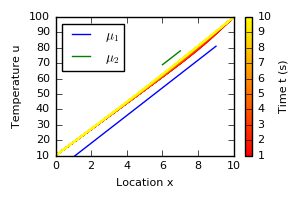
\includegraphics[width=0.49\textwidth]{ex2_plots0.png}}
        \hfill
    \subfloat[$a = 5.0, b = 20.0 $]{\label{fig:ex2_b}
        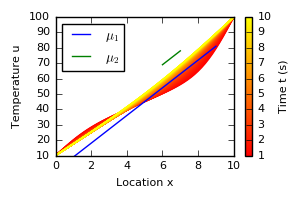
\includegraphics[width=0.49\textwidth]{ex2_plots1.png}}
        \hfill
        \caption{Two sample trajectories of $u^d(x, t)$ using a mesh of size
        $h=0.2$ and the reference profiles $\mu_1 = 9x$ and $\mu_2 = 9x + 15$}
    \label{fig:ex2_evolution}
\end{figure}


We show in Fig~\ref{fig:res_diffs} the difference between the true robustness and
the robustness for our mesh, both with and without the perturbations. Note that
when we include all perturbations, the computed robustness is less than the true
robustness, hence we correctly verify as satisfying all examples
that are satisfying. Regarding the conservatism of the approach, we obtain a
difference of at most 5.5 degrees in the robustness, which would allow us to verify a
specification that is satisfied by at least 5.5 degrees at all points in a system
that ranges through 90 degrees. It took an average of 19.29 seconds with a
standard deviation of 1.00 to verify the perturbed formula.

\begin{figure}
    \centering
    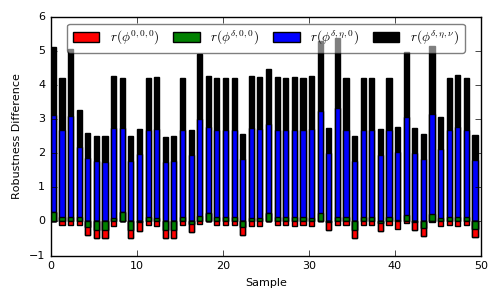
\includegraphics[width=0.8\linewidth]{figures/cs_ran_init_results.png}
    \caption{Difference between true robustness and robustness of the
        discretized specification with and without perturbations for
        random initial values}
    \label{fig:res_diffs}
\end{figure}


Finally, we verified the specification for sets of initial conditions of the
form $u_0(x) = a x + b$ with $a$ and $b$ constrained as before. Again we use a
mesh of size $h = 0.2$. We summarize our results in Table~\ref{tab:res_sets}.

\begin{table}
\centering
\begin{tabular}{|c|c|c|c|c|}
    \hline
    $a$ & $b$ & Minimum robustness & Result & Time (s)  \\
    \hline
    9 & [5, 13] & 0.5 & Satisfies & 21 \\
    9 & [5, 15] & -0.7 & Undefined & 22 \\
    9 & [0, 10] & -2.8 & Undefined & 22 \\
    $[8, 10]$ & [5, 13] & -5.0 & Undefined & 379 \\
    $[8.5, 9.5]$ & [8, 10] & 0.5 & Satisfies & 326 \\
    $[5, 12]$ & [0, 20] & -29.6 & Undefined & 82 \\
    \hline
\end{tabular}
\caption{Verification of sets of initial values}
\label{tab:res_sets}
\end{table}

\section{Conclusion}
\label{sec:conclusion}


\end{document}
